\section{Xây dựng ứng dụng Android với React Native}

\subsection{Thiết lập môi trường}
Để bắt đầu xây dựng một ứng React Native, ta cần cài đặt môi trường lập trình trên thiết bị của mình. Cụ thể cần: NodeJS, JDK, ReactNativeCLI, Android Studio.
\subsubsection{NodeJS}
\begin{enumerate}
    \item[\textit{a.}] {\textit{Khái niệm}}\\
    NodeJS là một nền tảng (flatform) cung cấp môi trường runtime chạy JavaScript, được sử dụng để chạy các ứng dụng web bên ngoài client. Nền tảng này được phát triển bởi Ryan Dahl vào năm 2009, được xem là một giải pháp hoàn hảo cho các ứng dụng sử dụng nhiều dữ liệu nhờ vào mô hình hướng sự kiện (event-driven) không đồng bộ.
    \item[\textit{b.}] {\textit{Chức năng đối với React Native App}}\\
    NodeJS cung cấp các package để xây dựng ứng dụng React Native.
    \item[\textit{c.}] {\textit{Cài đặt}}\\
    Link cài đặt: \url{https://nodejs.org/en/download/}\\
    Có thể cài bằng các dòng lệnh thông qua terminal (phụ thuộc vào hệ điều hành của thiết bị):
    \begin{enumerate}
        \item[-] {Windows}: choco install -y nodejs-lts
        \item[-] {MacOS}: brew install node | brew install watchman
        \item[-] {Linux}: apk add nodejs npm
    \end{enumerate}
    Sau khi cài đặt xong, có thể kiểm tra lại bằng cách chạy dòng lệnh trong terminal:
    \begin{figure}[!ht]
        \centering
        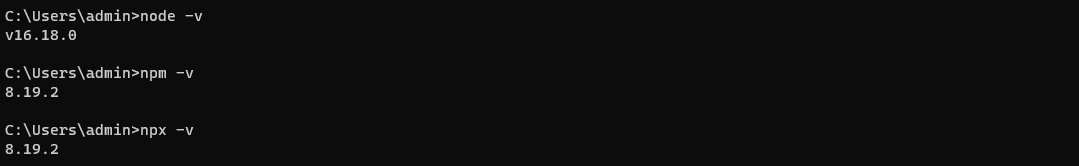
\includegraphics[scale=0.5]{images/checkNodeJS.png}
    \end{figure}
\end{enumerate}
\subsubsection{JDK}
\begin{enumerate}
    \item[\textit{a.}] {\textit{Khái niệm}}\\
    JDK (Java Development Kit) là một trong ba gói công nghệ cốt lõi được sử dụng trong lập trình Java: JVM (Máy ảo Java - Java Virtual Machine), JRE (Java Runtime Enviroment - Môi trường Java Runtime), JDK.\\
    Có thể định nghĩa JDK theo 2 cách sau:
    \begin{enumerate}
        \item[-] {\textit{Định nghĩa chuyển ngành}}: JDK là một hệ tiêu chuẩn trong việc triển khai nền tảng Java, bao gồm các trình thông dịch và thư viện lớp.
        \item[-] {\textit{Định nghĩa thông thường}}: JDK là gói phần mềm bạn tải xuống để tạo các ứng dụng dựa trên Java.
    \end{enumerate}
    \item[\textit{b.}] {\textit{Chức năng đối với React Native App}}\\
    Như đã trình bày ở phần kiến trúc Android, tầng Android Runtime cần trình biên dịch Java để compile ra các lớp.
    \item[\textit{c.}] {\textit{Cài đặt}}\\
    Link cài đặt: \url{https://www.oracle.com/eg/java/technologies/downloads/}\\
    Có thể cài bằng các dòng lệnh thông qua terminal (phụ thuộc vào hệ điều hành của thiết bị):
    \begin{enumerate}
        \item[-] {Windows}: choco install -y microsoft-openjdk11
        \item[-] {MacOS}: brew install java
        \item[-] {Linux}: sudo apt install default-jdk
    \end{enumerate}
    Sau khi cài đặt xong, có thể kiểm tra lại bằng cách chạy dòng lệnh trong terminal:
    \begin{figure}[!ht]
        \centering
        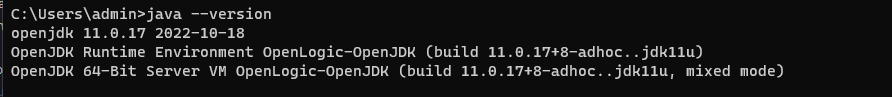
\includegraphics[scale=0.5]{images/checkJDK.png}
    \end{figure}
\end{enumerate}
% \subsubsection{ReactNativeCLI}
\subsubsection{Android Studio}
\begin{enumerate}
    \item[\textit{a.}] {\textit{Khái niệm}}\\
    Android Studio là IDE chính thức được sử dụng trong phát triển ứng dụng Android dựa trên IntelliJ IDEA.\\
    
    \item[] 
\end{enumerate}

\subsection{Xây dựng chương trình đầu tiên}

\subsection{Các khái niệm, thành phần}

\subsection{Một số thư viện phổ biến}

\subsection{Phát hành ứng dụng}
